\begin{figure*}[t]
\centering
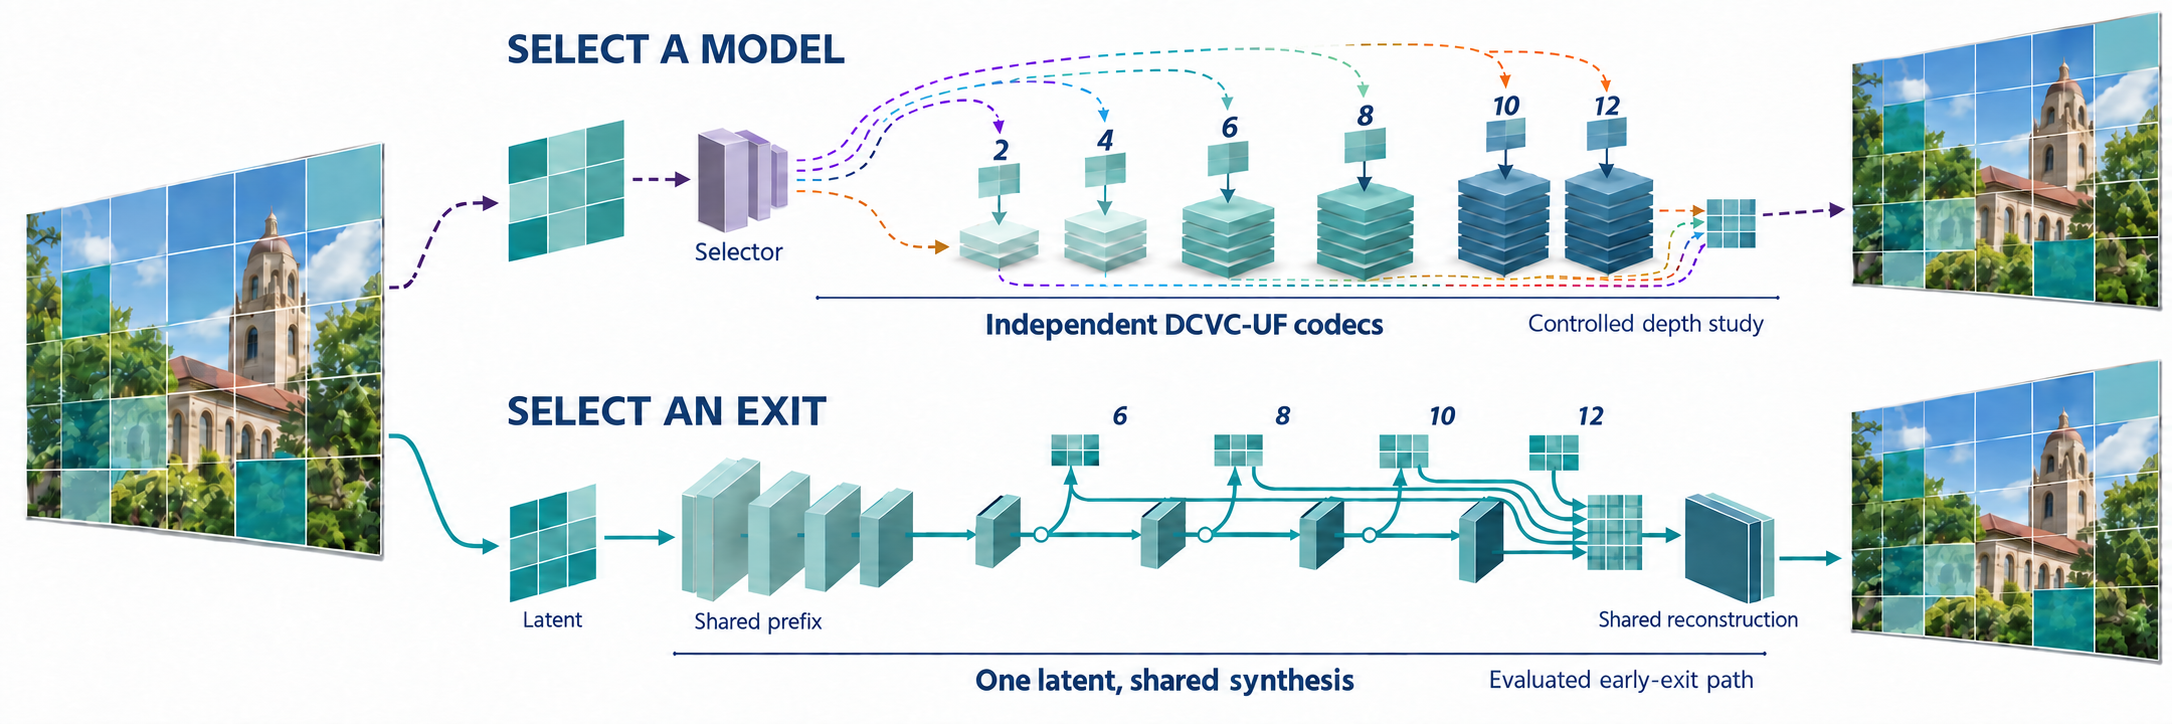
\includegraphics[width=\textwidth]{figs/adaptive20260927/adaptive_overview.png}
\caption{\textbf{One allocation principle, two ways to vary synthesis depth.}
\emph{Top:} select a complete DCVC-UF codec before encoding a patch; the
six-depth bank and its selector form the controlled, prospective study.
\emph{Bottom:} select a stopping depth within one shared-latent decoder;
this is the evaluated early-exit path. The paths are alternatives, not
successive stages. AI-generated conceptual illustration: picture planes
are illustrative, not dataset samples or reconstructed outputs. Exact
execution and measured allocations appear in \cref{fig:system,fig:maps}.}
\label{fig:overview}
\end{figure*}

\section{Introduction}
\label{sec:intro}

Efficient decoding is important for practical learned image compression.
Previous work has reduced decoder computation through shallow synthesis
transforms~\cite{yang2023shallow}, adaptive network width~\cite{hu2023cgslimdecoder}, and spatially dynamic
transforms~\cite{tao2023adanic}. Recent neural codecs further improve
practical efficiency by reducing memory traffic and function-call
overhead~\cite{jia2025dcvcrt} and simplifying entropy coding and
reconstruction~\cite{li2026dcvcuf}. These approaches make decoding
cheaper, but most computation is still determined by a fixed decoder
architecture.

The benefit of additional decoding, however, varies across an image.
Some regions improve substantially with deeper synthesis, while others
change little. Similar spatial variation has been exploited in
super-resolution by assigning patches to networks of different
capacities~\cite{kong2021classsr} or allowing them to exit at different
depths~\cite{wang2022ape}. Learned image compression introduces an
additional constraint: the reconstruction network operates on a coded
representation, making the choice of decoder capacity dependent on both
the synthesis transform and the representation it receives.

We propose \textbf{RegLIC}, a region-adaptive framework that assigns
different synthesis depths to different image regions. We study RegLIC
using the intra model of DCVC-UF~\cite{li2026dcvcuf}. DCVC-UF provides
a useful basis for this study because its synthesis transform contains
twelve constant-width blocks between upsampling and reconstruction.
This exposes decoder depth as a direct computation axis while retaining
the same feature width and synthesis structure. RegLIC uses this axis to
spend additional synthesis computation only on regions that benefit from
deeper processing.

We investigate two forms of region-adaptive depth
(\cref{fig:overview}). In the first, regions exit a shared synthesis
network at different depths. A common coded representation and synthesis
prefix are reused across all regions, while only surviving regions
execute later blocks. In the second, regions are assigned to independently
trained codecs with different decoder depths. Each codec learns its own
analysis, entropy, and synthesis transforms, allowing the coded
representation itself to specialize to decoder complexity. These two
settings compare shared computation with independent depth specialization
under the same spatial allocation principle.

For shared early exit, RegLIC divides the DCVC-UF synthesis transform
into a full-frame stem followed by conditional stages. Exited regions
are removed from subsequent computation, progressively reducing the
active workload. Exit adapters align features produced at different
depths before they are assembled and processed by a shared full-frame
reconstruction head. This allows one coded representation to support
different synthesis depths across an image without evaluating every
candidate depth.

Our key contributions are as follows:
\begin{itemize}
    \item We propose \textbf{RegLIC}, a region-adaptive learned image
    compression framework that allocates synthesis depth spatially. We
    study both shared early exits and selection among independently
    trained codecs with different decoder depths.

    \item We develop a shared-latent early-exit design for DCVC-UF that
    executes deeper synthesis blocks only for surviving regions and
    reconstructs features from different depths through a common output
    path.

    \item We demonstrate that region-adaptive depth reduces synthesis
    computation while preserving reconstruction quality, and isolate the
    benefit of spatial depth allocation from the reduction obtained by
    using shallower decoding alone.
\end{itemize}